\documentclass{standalone}
\usepackage{graphicx}	
\usepackage{amssymb, amsmath, amsthm}
\usepackage{color}

\usepackage{tikz}
\usetikzlibrary{intersections, backgrounds, math, arrows.meta}

\definecolor{light}{RGB}{220, 188, 188}
\definecolor{mid}{RGB}{185, 124, 124}
\definecolor{dark}{RGB}{143, 39, 39}
\definecolor{highlight}{RGB}{180, 31, 180}
\definecolor{darkteal}{RGB}{29, 79, 79}
\definecolor{darkolive}{RGB}{97, 123, 45}
\definecolor{gray10}{gray}{0.1}
\definecolor{gray20}{gray}{0.2}
\definecolor{gray30}{gray}{0.3}
\definecolor{gray40}{gray}{0.4}
\definecolor{gray60}{gray}{0.6}
\definecolor{gray70}{gray}{0.7}
\definecolor{gray80}{gray}{0.8}
\definecolor{gray90}{gray}{0.9}
\definecolor{gray95}{gray}{0.95}

\begin{document}

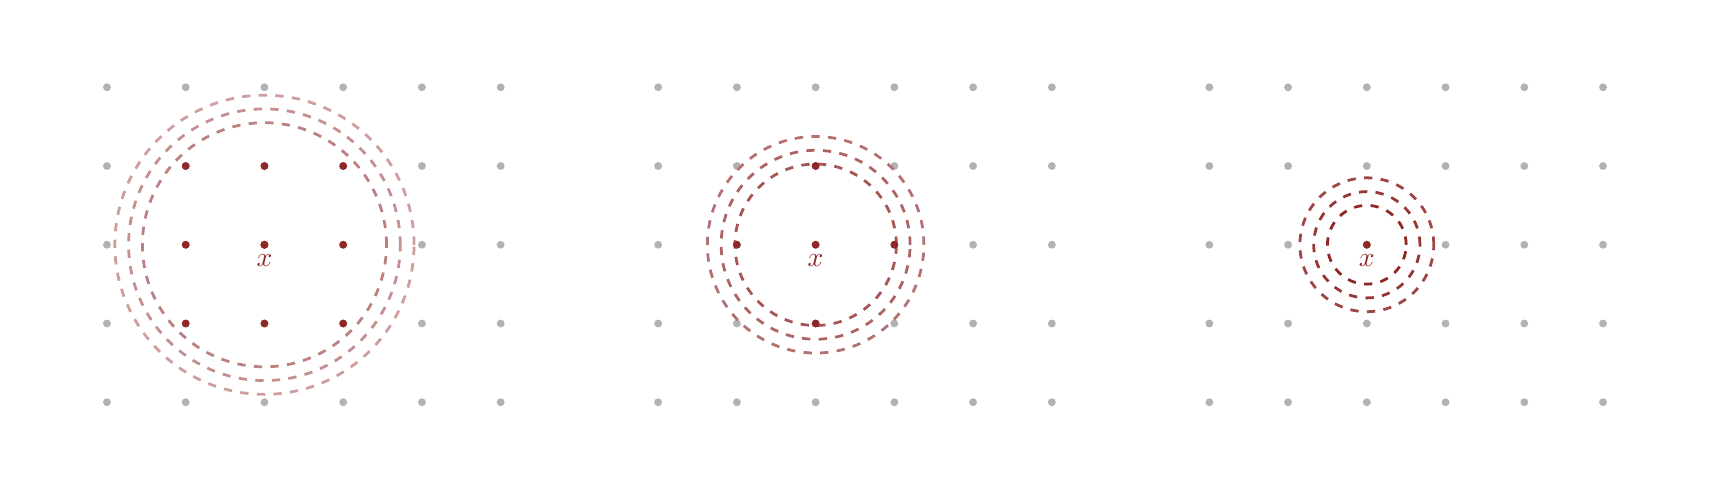
\begin{tikzpicture}[scale=1.0]
  
  \begin{scope}[shift={(0, 0)}]
    \draw[white] (-3.5, -2.75) rectangle (3.5, 2.75);
  
    \foreach \x in {-2.5, -1.5, ..., 2.5} {
      \foreach \y in {-2, -1, ..., 2} {
        \fill[gray70] (\x, \y) circle (0.05);
      }
    }
  
    \foreach \n in {2, 3, 4} {
      \pgfmathsetmacro{\r}{2.25 - \n * 1.75 / 10}
      \pgfmathsetmacro{\prop}{100 * \n / 10}
      \colorlet{custom}{dark!\prop!light}; 
      \draw[custom, dashed, line width=1] (-0.5, 0) circle (\r); 
    }
    
    \foreach \x in {-1.5, -0.5, +0.5} {
      \foreach \y in {-1, 0, +1} {
        \fill[dark] (\x, \y) circle (0.05);
      }
    }
  
    \fill[dark] (-0.5, 0) circle (0.05) node[below] { $x$ };
  \end{scope} 

  \begin{scope}[shift={(7, 0)}]
    \draw[white] (-3.5, -2.75) rectangle (3.5, 2.75);
  
    \foreach \x in {-2.5, -1.5, ..., 2.5} {
      \foreach \y in {-2, -1, ..., 2} {
        \fill[gray70] (\x, \y) circle (0.05);
      }
    }
  
    \foreach \n in {5, 6, 7} {
      \pgfmathsetmacro{\r}{2.25 - \n * 1.75 / 10}
      \pgfmathsetmacro{\prop}{100 * \n / 10}
      \colorlet{custom}{dark!\prop!light}; 
      \draw[custom, dashed, line width=1] (-0.5, 0) circle (\r); 
    }
  
    \fill[dark] (-0.5, +1) circle (0.05);
    \fill[dark] (-0.5, -1) circle (0.05);
    \fill[dark] (-1.5, 0) circle (0.05);
    \fill[dark] (+0.5, 0) circle (0.05);
    
    \fill[dark] (-0.5, 0) circle (0.05) node[below] { $x$ };
  \end{scope} 
  
  \begin{scope}[shift={(14, 0)}]
    \draw[white] (-3.5, -2.75) rectangle (3.5, 2.75);
  
    \foreach \x in {-2.5, -1.5, ..., 2.5} {
      \foreach \y in {-2, -1, ..., 2} {
        \fill[gray70] (\x, \y) circle (0.05);
      }
    }
  
    \foreach \n in {8, 9, ..., 10} {
      \pgfmathsetmacro{\r}{2.25 - \n * 1.75 / 10}
      \pgfmathsetmacro{\prop}{100 * \n / 10}
      \colorlet{custom}{dark!\prop!light}; 
      \draw[custom, dashed, line width=1] (-0.5, 0) circle (\r); 
    }
  
    \fill[dark] (-0.5, 0) circle (0.05) node[below] { $x$ };
  \end{scope} 
    
\end{tikzpicture}

\end{document}  